\documentclass[10pt]{article}
\usepackage{tikz}
\usetikzlibrary{shapes.misc}
\usepackage[margin=0cm]{geometry}
\pagestyle{empty}
\tikzstyle{every node}=[cross out, draw, red]

\begin{document}

\vspace*{\fill}
\begin{center}
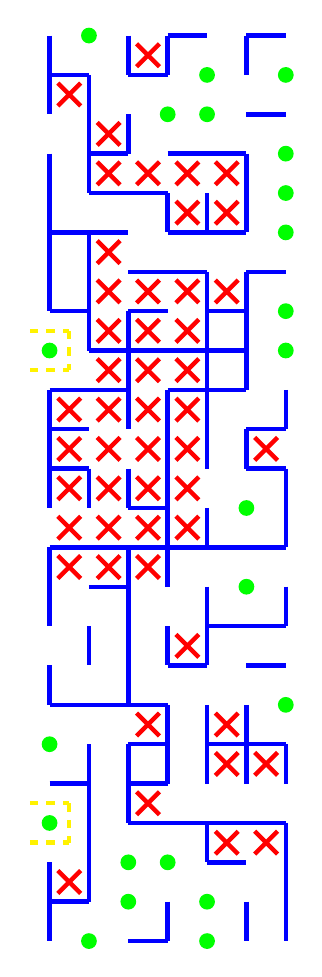
\begin{tikzpicture}[x=0.5cm, y=-0.5cm, ultra thick, blue]
% Walls
    \draw (3,0) -- (4,0);
    \draw (5,0) -- (6,0);
    \draw (0,1) -- (1,1);
    \draw (2,1) -- (3,1);
    \draw (5,2) -- (6,2);
    \draw (1,3) -- (2,3);
    \draw (3,3) -- (5,3);
    \draw (1,4) -- (3,4);
    \draw (0,5) -- (2,5);
    \draw (3,5) -- (5,5);
    \draw (2,6) -- (4,6);
    \draw (5,6) -- (6,6);
    \draw (0,7) -- (1,7);
    \draw (2,7) -- (3,7);
    \draw (4,7) -- (5,7);
    \draw (1,8) -- (5,8);
    \draw (0,9) -- (2,9);
    \draw (3,9) -- (5,9);
    \draw (0,10) -- (1,10);
    \draw (5,10) -- (6,10);
    \draw (0,11) -- (1,11);
    \draw (5,11) -- (6,11);
    \draw (2,12) -- (3,12);
    \draw (0,13) -- (6,13);
    \draw (1,14) -- (2,14);
    \draw (4,15) -- (6,15);
    \draw (3,16) -- (4,16);
    \draw (5,16) -- (6,16);
    \draw (0,17) -- (3,17);
    \draw (2,18) -- (3,18);
    \draw (4,18) -- (6,18);
    \draw (0,19) -- (1,19);
    \draw (2,19) -- (3,19);
    \draw (2,20) -- (6,20);
    \draw (4,21) -- (5,21);
    \draw (0,22) -- (1,22);
    \draw (2,23) -- (3,23);
    \draw (0,0) -- (0,2);
    \draw (0,3) -- (0,7);
    \draw (0,9) -- (0,12);
    \draw (0,13) -- (0,15);
    \draw (0,16) -- (0,17);
    \draw (0,21) -- (0,23);
    \draw (1,1) -- (1,4);
    \draw (1,5) -- (1,8);
    \draw (1,11) -- (1,12);
    \draw (1,15) -- (1,16);
    \draw (1,18) -- (1,22);
    \draw (2,0) -- (2,1);
    \draw (2,2) -- (2,3);
    \draw (2,7) -- (2,10);
    \draw (2,11) -- (2,12);
    \draw (2,13) -- (2,17);
    \draw (2,18) -- (2,20);
    \draw (3,0) -- (3,1);
    \draw (3,4) -- (3,5);
    \draw (3,9) -- (3,14);
    \draw (3,15) -- (3,16);
    \draw (3,17) -- (3,19);
    \draw (3,22) -- (3,23);
    \draw (4,4) -- (4,5);
    \draw (4,6) -- (4,11);
    \draw (4,12) -- (4,13);
    \draw (4,14) -- (4,16);
    \draw (4,17) -- (4,19);
    \draw (4,20) -- (4,21);
    \draw (5,0) -- (5,1);
    \draw (5,3) -- (5,5);
    \draw (5,6) -- (5,9);
    \draw (5,10) -- (5,11);
    \draw (5,17) -- (5,19);
    \draw (5,22) -- (5,23);
    \draw (6,9) -- (6,10);
    \draw (6,11) -- (6,13);
    \draw (6,14) -- (6,15);
    \draw (6,18) -- (6,19);
    \draw (6,20) -- (6,23);
% Pillars
    \fill[green] (1,0) circle(0.2);
    \fill[green] (4,1) circle(0.2);
    \fill[green] (6,1) circle(0.2);
    \fill[green] (3,2) circle(0.2);
    \fill[green] (4,2) circle(0.2);
    \fill[green] (6,3) circle(0.2);
    \fill[green] (6,4) circle(0.2);
    \fill[green] (6,5) circle(0.2);
    \fill[green] (6,7) circle(0.2);
    \fill[green] (0,8) circle(0.2);
    \fill[green] (6,8) circle(0.2);
    \fill[green] (5,12) circle(0.2);
    \fill[green] (5,14) circle(0.2);
    \fill[green] (6,17) circle(0.2);
    \fill[green] (0,18) circle(0.2);
    \fill[green] (0,20) circle(0.2);
    \fill[green] (2,21) circle(0.2);
    \fill[green] (3,21) circle(0.2);
    \fill[green] (2,22) circle(0.2);
    \fill[green] (4,22) circle(0.2);
    \fill[green] (1,23) circle(0.2);
    \fill[green] (4,23) circle(0.2);
% Inner points in accessible cul-de-sacs
    \node at (2.5,0.5) {};
    \node at (0.5,1.5) {};
    \node at (1.5,2.5) {};
    \node at (1.5,3.5) {};
    \node at (2.5,3.5) {};
    \node at (3.5,3.5) {};
    \node at (4.5,3.5) {};
    \node at (3.5,4.5) {};
    \node at (4.5,4.5) {};
    \node at (1.5,5.5) {};
    \node at (1.5,6.5) {};
    \node at (2.5,6.5) {};
    \node at (3.5,6.5) {};
    \node at (4.5,6.5) {};
    \node at (1.5,7.5) {};
    \node at (2.5,7.5) {};
    \node at (3.5,7.5) {};
    \node at (1.5,8.5) {};
    \node at (2.5,8.5) {};
    \node at (3.5,8.5) {};
    \node at (0.5,9.5) {};
    \node at (1.5,9.5) {};
    \node at (2.5,9.5) {};
    \node at (3.5,9.5) {};
    \node at (0.5,10.5) {};
    \node at (1.5,10.5) {};
    \node at (2.5,10.5) {};
    \node at (3.5,10.5) {};
    \node at (5.5,10.5) {};
    \node at (0.5,11.5) {};
    \node at (1.5,11.5) {};
    \node at (2.5,11.5) {};
    \node at (3.5,11.5) {};
    \node at (0.5,12.5) {};
    \node at (1.5,12.5) {};
    \node at (2.5,12.5) {};
    \node at (3.5,12.5) {};
    \node at (0.5,13.5) {};
    \node at (1.5,13.5) {};
    \node at (2.5,13.5) {};
    \node at (3.5,15.5) {};
    \node at (2.5,17.5) {};
    \node at (4.5,17.5) {};
    \node at (4.5,18.5) {};
    \node at (5.5,18.5) {};
    \node at (2.5,19.5) {};
    \node at (4.5,20.5) {};
    \node at (5.5,20.5) {};
    \node at (0.5,21.5) {};
% Entry-exit paths without intersections
    \draw[dashed, yellow] (-0.5,7.5) -- (0.5,7.5);
    \draw[dashed, yellow] (-0.5,8.5) -- (0.5,8.5);
    \draw[dashed, yellow] (-0.5,19.5) -- (0.5,19.5);
    \draw[dashed, yellow] (-0.5,20.5) -- (0.5,20.5);
    \draw[dashed, yellow] (0.5,7.5) -- (0.5,8.5);
    \draw[dashed, yellow] (0.5,19.5) -- (0.5,20.5);
\end{tikzpicture}
\end{center}
\vspace*{\fill}

\end{document}
